\documentclass[a4paper,12pt,twoside]{memoir}

% Castellano
\usepackage[spanish,es-tabla]{babel}
\selectlanguage{spanish}
\usepackage[utf8]{inputenc}
\usepackage[T1]{fontenc}
\usepackage{lmodern} % scalable font
\usepackage{microtype}
\usepackage{placeins}
\usepackage{graphicx}
\usepackage{subcaption}

\RequirePackage{booktabs}
\RequirePackage[table]{xcolor}
\RequirePackage{xtab}
\RequirePackage{multirow}

% Links
\usepackage[colorlinks]{hyperref}
\hypersetup{
	allcolors = {red}
}

% Ecuaciones
\usepackage{amsmath}

% Rutas de fichero / paquete
\newcommand{\ruta}[1]{{\sffamily #1}}

% Párrafos
\nonzeroparskip


% Imagenes
\usepackage{graphicx}
\newcommand{\imagen}[2]{
	\begin{figure}[!h]
		\centering
		\includegraphics[width=0.9\textwidth]{#1}
		\caption{#2}\label{fig:#1}
	\end{figure}
	\FloatBarrier
}

\newcommand{\imagenflotante}[2]{
	\begin{figure}%[!h]
		\centering
		\includegraphics[width=0.9\textwidth]{#1}
		\caption{#2}\label{fig:#1}
	\end{figure}
}



% El comando \figura nos permite insertar figuras comodamente, y utilizando
% siempre el mismo formato. Los parametros son:
% 1 -> Porcentaje del ancho de página que ocupará la figura (de 0 a 1)
% 2 --> Fichero de la imagen
% 3 --> Texto a pie de imagen
% 4 --> Etiqueta (label) para referencias
% 5 --> Opciones que queramos pasarle al \includegraphics
% 6 --> Opciones de posicionamiento a pasarle a \begin{figure}
\newcommand{\figuraConPosicion}[6]{%
  \setlength{\anchoFloat}{#1\textwidth}%
  \addtolength{\anchoFloat}{-4\fboxsep}%
  \setlength{\anchoFigura}{\anchoFloat}%
  \begin{figure}[#6]
    \begin{center}%
      \Ovalbox{%
        \begin{minipage}{\anchoFloat}%
          \begin{center}%
            \includegraphics[width=\anchoFigura,#5]{#2}%
            \caption{#3}%
            \label{#4}%
          \end{center}%
        \end{minipage}
      }%
    \end{center}%
  \end{figure}%
}

%
% Comando para incluir imágenes en formato apaisado (sin marco).
\newcommand{\figuraApaisadaSinMarco}[5]{%
  \begin{figure}%
    \begin{center}%
    \includegraphics[angle=90,height=#1\textheight,#5]{#2}%
    \caption{#3}%
    \label{#4}%
    \end{center}%
  \end{figure}%
}
% Para las tablas
\newcommand{\otoprule}{\midrule [\heavyrulewidth]}
%
% Nuevo comando para tablas pequeñas (menos de una página).
\newcommand{\tablaSmall}[5]{%
 \begin{table}
  \begin{center}
   \rowcolors {2}{gray!35}{}
   \begin{tabular}{#2}
    \toprule
    #4
    \otoprule
    #5
    \bottomrule
   \end{tabular}
   \caption{#1}
   \label{tabla:#3}
  \end{center}
 \end{table}
}

%
%Para el float H de tablaSmallSinColores
\usepackage{float}

%
% Nuevo comando para tablas pequeñas (menos de una página).
\newcommand{\tablaSmallSinColores}[5]{%
 \begin{table}[H]
  \begin{center}
   \begin{tabular}{#2}
    \toprule
    #4
    \otoprule
    #5
    \bottomrule
   \end{tabular}
   \caption{#1}
   \label{tabla:#3}
  \end{center}
 \end{table}
}

\newcommand{\tablaApaisadaSmall}[5]{%
\begin{landscape}
  \begin{table}
   \begin{center}
    \rowcolors {2}{gray!35}{}
    \begin{tabular}{#2}
     \toprule
     #4
     \otoprule
     #5
     \bottomrule
    \end{tabular}
    \caption{#1}
    \label{tabla:#3}
   \end{center}
  \end{table}
\end{landscape}
}

%
% Nuevo comando para tablas grandes con cabecera y filas alternas coloreadas en gris.
\newcommand{\tabla}[6]{%
  \begin{center}
    \tablefirsthead{
      \toprule
      #5
      \otoprule
    }
    \tablehead{
      \multicolumn{#3}{l}{\small\sl continúa desde la página anterior}\\
      \toprule
      #5
      \otoprule
    }
    \tabletail{
      \hline
      \multicolumn{#3}{r}{\small\sl continúa en la página siguiente}\\
    }
    \tablelasttail{
      \hline
    }
    \bottomcaption{#1}
    \rowcolors {2}{gray!35}{}
    \begin{xtabular}{#2}
      #6
      \bottomrule
    \end{xtabular}
    \label{tabla:#4}
  \end{center}
}

%
% Nuevo comando para tablas grandes con cabecera.
\newcommand{\tablaSinColores}[6]{%
  \begin{center}
    \tablefirsthead{
      \toprule
      #5
      \otoprule
    }
    \tablehead{
      \multicolumn{#3}{l}{\small\sl continúa desde la página anterior}\\
      \toprule
      #5
      \otoprule
    }
    \tabletail{
      \hline
      \multicolumn{#3}{r}{\small\sl continúa en la página siguiente}\\
    }
    \tablelasttail{
      \hline
    }
    \bottomcaption{#1}
    \begin{xtabular}{#2}
      #6
      \bottomrule
    \end{xtabular}
    \label{tabla:#4}
  \end{center}
}

%
% Nuevo comando para tablas grandes sin cabecera.
\newcommand{\tablaSinCabecera}[5]{%
  \begin{center}
    \tablefirsthead{
      \toprule
    }
    \tablehead{
      \multicolumn{#3}{l}{\small\sl continúa desde la página anterior}\\
      \hline
    }
    \tabletail{
      \hline
      \multicolumn{#3}{r}{\small\sl continúa en la página siguiente}\\
    }
    \tablelasttail{
      \hline
    }
    \bottomcaption{#1}
  \begin{xtabular}{#2}
    #5
   \bottomrule
  \end{xtabular}
  \label{tabla:#4}
  \end{center}
}



\definecolor{cgoLight}{HTML}{EEEEEE}
\definecolor{cgoExtralight}{HTML}{FFFFFF}

%
% Nuevo comando para tablas grandes sin cabecera.
\newcommand{\tablaSinCabeceraConBandas}[5]{%
  \begin{center}
    \tablefirsthead{
      \toprule
    }
    \tablehead{
      \multicolumn{#3}{l}{\small\sl continúa desde la página anterior}\\
      \hline
    }
    \tabletail{
      \hline
      \multicolumn{#3}{r}{\small\sl continúa en la página siguiente}\\
    }
    \tablelasttail{
      \hline
    }
    \bottomcaption{#1}
    \rowcolors[]{1}{cgoExtralight}{cgoLight}

  \begin{xtabular}{#2}
    #5
   \bottomrule
  \end{xtabular}
  \label{tabla:#4}
  \end{center}
}




\graphicspath{ {./img/} }

% Capítulos
\chapterstyle{bianchi}
\newcommand{\capitulo}[2]{
	\setcounter{chapter}{#1}
	\setcounter{section}{0}
	\chapter*{#2}
	\addcontentsline{toc}{chapter}{#2}
	\markboth{#2}{#2}
}

% Apéndices
\renewcommand{\appendixname}{Apéndice}
\renewcommand*\cftappendixname{\appendixname}

\newcommand{\apendice}[1]{
	%\renewcommand{\thechapter}{A}
	\chapter{#1}
}

\renewcommand*\cftappendixname{\appendixname\ }

% Formato de portada
\makeatletter
\usepackage{xcolor}
\newcommand{\tutor}[1]{\def\@tutor{#1}}
\newcommand{\course}[1]{\def\@course{#1}}
\definecolor{cpardoBox}{HTML}{E6E6FF}
\def\maketitle{
  \null
  \thispagestyle{empty}
  % Cabecera ----------------
\noindent
\includegraphics[width=\textwidth]{cabecera}\vspace{1cm}%
  \vfill
  % Título proyecto y escudo informática ----------------
  \colorbox{cpardoBox}{%
    \begin{minipage}{.8\textwidth}
      \vspace{.5cm}\Large
      \begin{center}
      \textbf{TFG del Grado en Ingeniería Informática}\vspace{.6cm}\\
      \textbf{\LARGE\@title{}}
      \end{center}
      \vspace{.2cm}
    \end{minipage}

  }%
  \hfill\begin{minipage}{.20\textwidth}
    
\includegraphics[width=\textwidth]{escudoInfor}
  \end{minipage}
  \vfill
  % Datos de alumno, curso y tutores ------------------
  \begin{center}%
  {%
    \noindent\LARGE
    Presentado por \@author{}\\ 
    en Universidad de Burgos --- \@date{}\\
    Tutor: \@tutor{}\\
  }%
  \end{center}%
  \null
  \cleardoublepage
  }
\makeatother


% Datos de portada
\title{título del TFG \\Documentación Técnica}
\author{nombre alumno}
\tutor{nombre tutor}
\date{\today}

\begin{document}

\maketitle



\cleardoublepage



%%%%%%%%%%%%%%%%%%%%%%%%%%%%%%%%%%%%%%%%%%%%%%%%%%%%%%%%%%%%%%%%%%%%%%%%%%%%%%%%%%%%%%%%



\frontmatter


\clearpage

% Indices
\tableofcontents

\clearpage

\listoffigures

\clearpage

\listoftables

\clearpage

\mainmatter

\appendix

\apendice{Plan de Proyecto Software}

\section{Introducción}
%Ref david goo bees https://github.com/davidmigloz/go-bees puede ayudar con la memoria
El plan del proyecto es un documento que recoge el tiempo, esfuerzo y el dinero que supondrá la realización del proyecto.
Este plan se divide en dos partes:
\begin{itemize}
	\tightlist
	\item Planificación temporal
	\item Estudio de la viabilidad
\end{itemize}
El objetivo de la primera es estimar el tiempo y el esfuerzo que se requieren para la realización del proyecto, 
La segunda parte se centra en un análisis de la viabilidad del proyecto. Se objetivo es estimar si el proyecto se podría realizar con éxito. El análisis de viabilidad se puede ha dividido en dos apartados:
\begin{description}
	\tightlist
	\item[Viabilidad económica]: Análisis del coste y del beneficio que supondría la realización del proyecto.
	\item[Viabilidad legal]: Análisis de las leyes que se aplicarían desde el comienzo del proyecto.En un proyecto software tienen especial importancia las licencias y la Ley
	de Protección de Datos.
\end{description}

\section{Planificación temporal}
No se ha realizado una planificación temporal del proyecto. Pero se podría decir que se han tratado de seguir los 12 principios del manifiesto ágil y el modelo SCRUM \cite{noauthor_scrum_2019}:
\begin{itemize}
	\tightlist
	\item Se ha aplicado un desarrollo incremental y evolutivo.
	\item Se han realizado iteraciones (sprints) de dos semanas. Al finalizar un sprint se realizaba una reunión entre el tutor y el alumno que daba comienzo al siguiente sprint y que consta de dos partes:
	\begin{itemize}
		\item Una parte de revisión del sprint en la que se exponía una parte operativa del producto.
		\item Otra de planificación del siguiente sprint en la que se determinaba el trabajo y los objetivos a alcanzar durante el sprint siguiente. Esto quedaba reflejado como una pila de tareas que se debían completar durante el sprint y que han sido registradas en el sistema de gestión de incidencias de GitLab.
	\end{itemize}
\end{itemize}
\subsection{Sprints}
A continuación se definen los sprints y sus respectivas pilas de tareas que se llevaron a cabo durante la realización del proyecto. 
Se pueden visualizar las issues en orden ascendente de creación a partir de esta URL:

\subsubsection{Inicio del proyecto}
El proyecto comenzó el 1 de octubre de 2018. Las primeras tareas que se definieron fueron de investigación y configuración del entorno de trabajo, no se definían de forma muy clara ya que aun no se sabía que caminos escoger para la realización del proyecto.

\section{Estudio de viabilidad}

\subsection{Viabilidad económica}

\subsection{Viabilidad legal}



\apendice{Especificación de Requisitos}\label{anex:B}

\section{Introducción}

Este anexo tiene como objetivo analizar y documentar las necesidades funcionales y no funcionales que deberán ser soportadas por el software desarrollado.

%Para representar estas necesidades se utilizaran historias de usuario, que describen lo que el usuario debería poder hacer, en lugar de los tradicionales requisitos funcionales, que describen características más específicas del desarrollo del sistema de un modo más técnico. A menudo se recurrirá a diagramas de casos de uso, que describen todas las interacciones que tendrán los usuarios con el software.

\section{Objetivos generales}
El objetivo general de este TFG es diseñar una aplicación Web en Java que permita obtener un conjunto de métricas de evolución del proceso software a partir de repositorios de GitLab, para permitir comparar los distintos procesos de desarrollo software de cada repositorio. La aplicación se probará con datos reales para comparar los repositorios de Trabajos Fin de Grado del Grado de Ingeniería Informática presentados en GitLab. Con más detalle:
\begin{itemize}
	\tightlist
	\item Se obtendrán medidas de métricas de evolución de uno o varios proyectos alojados en repositorios de GitLab.
	\item Las métricas que se desean calcular de un repositorio  son algunas de las especificadas en la tesis titulada ``\textit{sPACE: Software Project Assessment in the Course of Evolution}'' \citep{ratzinger_space:_2007} y 
	adaptadas a los repositorios software:
	\begin{itemize}
		\tightlist
		\item Número total de incidencias (\textit{issues})
		\item Cambios (\textit{commits}) por incidencia
		\item Porcentaje de incidencias cerrados
		\item Media de días en cerrar una incidencia
		\item Media de días entre cambios
		\item Días entre primer y último cambio
		\item Rango de actividad de cambios por mes
		\item Porcentaje de pico de cambios
	\end{itemize}
	\item El objetivo de obtener las métricas es poder evaluar el estado de un proyecto comparándolo con otros proyectos de la misma naturaleza. Para ello se deberán establecer unos valores umbrales por cada métrica basados en el cálculo de los cuartiles Q1 y Q3. Además, estos valores se calcularán dinámicamente y se almacenarán en perfiles de configuración de métricas.
	\item Se dará la posibilidad de almacenar de manera persistente estos perfiles de métricas para permitir comparaciones futuras. Un ejemplo de utilidad es guardar los valores umbrales de repositorios por lenguaje de programación, o en el caso de repositorios de TFG de la UBU por curso académico.
	\item También se permitirá almacenar de forma persistente las métricas obtenidas de los repositorios para su posterior consulta o tratamiento. Esto permitiría comparar nuevos proyectos con proyectos de los que ya se han calculado sus métricas.
\end{itemize}

\section{Objetivos técnicos}
Este apartado resume requisitos del proyecto más técnicos y centrados en el proceso y otras características no funcionales.
\begin{itemize}
	\tightlist
	\item Diseñar la aplicación de manera que se puedan extender con nuevas métricas con el menor coste de mantenimiento posible. Para ello, se aplicará un diseño basado en frameworks y en patrones de diseño \citep{gamma_patrones_2002}.
	\item El diseño de la aplicación debe facilitar la extensión a otras plataformas de desarrollo colaborativo como GitHub o Bitbucket.
	\item Aplicar el \textit{frameworks `modelo-vista-controlador'} para separar la lógica de la aplicación y la interfaz de usuario.
	\item Crear una batería de pruebas automáticas con cobertura por encima del 90\% en los subsistemas de lógica de la aplicación.
	\item Utilizar una plataforma de desarrollo colaborativo que incluya un sistema de control de versiones, un sistema de seguimiento de incidencias y que permita una comunicación fluida entre el tutor y el alumno.
	\item Utilizar un sistema de integración y despliegue continuo.
	\item Diseñar una correcta gestión de errores definiendo excepciones de biblioteca y registrando eventos de error e información en ficheros de \textit{log}. 
	\item Aplicar nuevas estructuras  del lenguaje Java para el desarrollo, como son expresiones lambda. 
	\item Utilizar sistemas que aseguren la calidad continua del código que permitan evaluar la deuda técnica del proyecto.
	\item Probar la aplicación con ejemplos reales y utilizando técnicas avanzadas, como entrada de datos de test en ficheros con formato tabulado tipo CSV (\textit{Comma Separated Values}). 	
\end{itemize}

\section{Actores}
Se consideran dos actores: El usuario de la aplicación y el desarrollador. Además de poder ser utilizado por un usuario, la aplicación deberá estar preparada para que en un futuro se pueda extender en cuanto a número de métricas y forjas de repositorios.

\section{Catalogo de requisitos}
Este apartado enumera los diferentes requisitos que el sistema software deberá satisfacer. Se divide en dos apartados. El primero detalla los servicios que prestará el sistema al usuario final o a otros sistemas; el segundo detalla funciones más técnicas de cómo se desarrollará el proceso software y otras propiedades del sistema como eficiencia o mantenibilidad.

\subsection{Requisitos funcionales}

\begin{itemize}
	\item \textbf{RF-1} Establecer conexión con GitLab: El usuario debe poder establecer distintos tipos de conexión a GitLab.
	\begin{itemize}
		\item \textbf{RF-1.1} El usuario podrá iniciar sesión desde la aplicación mediante usuario y contraseña a su usuario en GitLab para poder obtener los repositorios públicos y privados a los que tenga acceso.
		\item \textbf{RF-1.2} El usuario podrá iniciar sesión desde la aplicación mediante un token de acceso personal a su usuario en GitLab para poder obtener los repositorios públicos y privados a los que tenga acceso.
		\item \textbf{RF-1.3} El usuario podrá establecer una conexión pública a GitLab para poder obtener los repositorios públicos.
		\item \textbf{RF-1.4} El usuario podrá utilizar la aplicación sin establecer una conexión. Aunque no tenga acceso a los repositorios de GitLab.
		\item \textbf{RF-1.5} El usuario deberá elegir un tipo de conexión al entrar por primera vez a la aplicación.
		\item \textbf{RF-1.6} La aplicación mostrará al usuario en todo momento la conexión que está utilizando
		\item \textbf{RF-1.7} El usuario podrá cambiar de conexión teniendo en cuenta que solo puede haber un tipo de conexión activo en un instante dado
	\end{itemize}
	\item \textbf{RF-2} Gestión de proyectos. El usuario podrá calcular las métricas de proyectos de GitLab definidas en la sección \ref{sect:B_5_1_1}: `\textit{Definición de las métricas}' y se mostrarán los resultados en forma de tabla en la que las filas se correspondan con los proyectos y las columnas con las métricas.
	\begin{itemize}
		\item \textbf{RF-2.1} El usuario podrá añadir un proyecto siempre que tenga una conexión a GitLab (con sesión o pública)
		\begin{itemize}
			\item \textbf{RF-2.1.1} El usuario podrá añadir un proyecto a partir del nombre de usuario o ID del propietario y el nombre del proyecto, siempre que tenga acceso desde la conexión establecida
			\item \textbf{RF-2.1.2} El usuario podrá añadir un proyecto a partir del nombre o del ID del grupo al que pertenece el proyecto y su nombre, siempre que tenga acceso desde la conexión establecida
			\item \textbf{RF-2.1.3} El usuario podrá añadir un proyecto a partir de su URL, siempre que tenga acceso desde la conexión establecida
		\end{itemize}
		\item \textbf{RF-2.2} El usuario no podrá añadir un proyecto que ya esté en la tabla
		\item \textbf{RF-2.3} Al añadir un proyecto a la tabla se calcularán las métricas definidas en la sección \ref{sect:B_5_1_1}: `\textit{Definición de las métricas}' y se mostrarán en forma de tabla.
		\item \textbf{RF-2.4} El usuario podrá eliminar un proyecto de la tabla
		\item \textbf{RF-2.5} El usuario podrá volver a obtener las métricas de un repositorio que ya haya añadido, siempre que tenga acceso desde la conexión establecida
		\item \textbf{RF-2.6} El usuario podrá exportar los proyectos y sus métricas a un fichero con formato `\ruta{.emr}'
		\item \textbf{RF-2.7} El usuario podrá exportar los resultados de las métricas de todos los proyectos en un fichero con formato CSV
		\item \textbf{RF-2.8} El usuario podrá importar y añadir repositorios a la tabla  desde un fichero con formato `\ruta{.emr}', respetando el requisito RF2.2 de no añadir un repositorio ya existente
		\item \textbf{RF-2.9} El usuario podrá importar repositorios a la tabla, sobrescribiendo los de la tabla.
		\item \textbf{RF-2.10} Se podrán filtrar los proyectos por su nombre
		\item \textbf{RF-2.11} Se puede ordenar los repositorios por nombre, fecha de medición y por cualquiera de las métricas
		\item \textbf{RF-2.12} Al ordenar por métricas habrá que tener en cuenta que habrá medidas que no se habrán calculado por falta de datos de GitLab
	\end{itemize}
	\item RF-3 Evaluación de métricas. Las métricas, una vez calculadas, serán evaluadas mediante un código de color (verde - bueno, naranja - peligro, rojo - malo) a partir de un perfil de métricas, que será un conjunto de valores mínimo y máximo de cada una de las métricas, a partir de la definición de la evaluación en la sección \ref{sect:B_5_1_2}: `\textit{Evaluación de métricas}'
	\begin{itemize}
		\item \textbf{RF-3.1} Se podrá cargar un perfil de métricas que contenga valores umbrales mínimo y máximo y se utilizarán para evaluarlas
		\item \textbf{RF-3.1} El usuario podrá cargar un perfil por defecto creado a partir de un conjunto de datos \footnote{\url{https://github.com/clopezno/clopezno.github.io/blob/master/agile_practices_experiment/DataSet_EvolutionSoftwareMetrics_FYP.csv}} de un estudio empírico de las métricas de evolución del software en trabajos finales de grado\cite{lopez_nozal_measuring_2019}
		\item \textbf{RF-3.2} El usuario podrá cargar un perfil creado a partir de los repositorios que existan en la tabla
		\item \textbf{RF-3.3} El usuario podrá exportar el perfil de métricas que tenga cargado a un fichero con formato \ruta{emmp}
		\item \textbf{RF-3.4} El usuario podrá importar un perfil de métricas que haya guardado anteriormente para evaluar los repositorios que tenga en la tabla
		\item \textbf{RF-3.5} En un instante, solo puede haber un perfil de métricas cargado
		\item \textbf{RF-3.6} Por defecto se cargará el perfil por defecto
	\end{itemize}
\end{itemize}

\subsubsection{Definición de las métricas}\label{sect:B_5_1_1}

En el requisito RF-2 se entiende que se debe calcular las siguientes métricas de un proyecto:

\textbf{\underline{I1 - Número total de issues (incidencias)}}

\begin{itemize}
	\item \textbf{Categoría}: Proceso de Orientación
	\item \textbf{Descripción}: Número total de issues creadas en el repositorio
	\item \textbf{Propósito}: ¿Cuántas issues se han definido en el repositorio?
	\item \textbf{Fórmula}: $NTI$. \textit{NTI = número total de issues}
	\item \textbf{Fuente de medición}: Proyecto en una plataforma de desarrollo colaborativo.
	\item \textbf{Interpretación}: $NTI \geq 0$. Valores bajos indican que no se utiliza un sistema de seguimiento de incidencias, podría ser porque el proyecto acaba de comenzar
	\item \textbf{Tipo de escala}: Absoluta
	\item \textbf{Tipo de medida}: \textit{NTI = Contador}
\end{itemize}

\textbf{\underline{I2 - Commits (cambios) por issue}}

\begin{itemize}
	\item \textbf{Categoría}: Proceso de Orientación
	\item \textbf{Descripción}: Número de commits por issue
	\item \textbf{Propósito}: ¿Cuál es el volumen medio de trabajo de las issues?
	\item \textbf{Fórmula}: $CI = \frac{NTC}{NTI}$. \textit{CI = Cambios por issue, NTC = Número total de commits, NTI = Numero total de issues}
	\item \textbf{Fuente de medición}: Proyecto en una plataforma de desarrollo colaborativo.
	\item \textbf{Interpretación}: $CI \geq 1$, Lo normal son valores altos. Si el valor es menor que uno significa que hay desarrollo sin documentar.
	\item \textbf{Tipo de escala}: Ratio 
	\item \textbf{Tipo de medida}: \textit{NTC, NTI = Contador}
\end{itemize}

\textbf{\underline{I3 - Porcentaje de issues cerradas}}

\begin{itemize}
	\item \textbf{Categoría}: Proceso de Orientación
	\item \textbf{Descripción}: Porcentaje de issues cerradas
	\item \textbf{Propósito}: ¿Qué porcentaje de issues definidas en el repositorio se han cerrado?
	\item \textbf{Fórmula}: $PIC = \frac{NTIC}{NTI}*100$. \textit{PIC = Porcentaje de issues cerradas, NTIC = Número total de issues cerradas, NTI = Numero total de issues}
	\item \textbf{Fuente de medición}: Proyecto en una plataforma de desarrollo colaborativo.
	\item \textbf{Interpretación}: $0 \leq PIC \leq 100$. Cuanto más alto mejor
	\item \textbf{Tipo de escala}: Ratio
	\item \textbf{Tipo de medida}: \textit{NTI, NTIC = Contador}
\end{itemize}

\textbf{\underline{TI1 - Media de días en cerrar una issue}}

\begin{itemize}
	\item \textbf{Categoría}: Constantes de tiempo
	\item \textbf{Descripción}:  Media de días en cerrar una issue
	\item \textbf{Propósito}: ¿Cuánto se suele tardar en cerrar una issue? 
	\item \textbf{Fórmula}: $MDCI = \frac{\sum_{i=0}^{NTIC}DCI_i}{NTIC}$. \textit{MDCI = Media de días en cerrar una issue, NTIC = Número total de issues cerradas, DCI = Días en cerrar la issue}
	\item \textbf{Fuente de medición}: Proyecto en una plataforma de desarrollo colaborativo.
	\item \textbf{Interpretación}: $MDCI \geq 0$. Cuanto más pequeño mejor. Si se siguen metodologías ágiles de desarrollo iterativo e incremental como SCRUM, la métrica debería indicar la duración del \textit{sprint} definido en la fase de planificación del proyecto. En SCRUM se recomiendan duraciones del \textit{sprint} de entre una y seis semanas, siendo recomendable que no exceda de un mes \citep{scrum_master_scrum_2019}.
	\item \textbf{Tipo de escala}: Ratio
	\item \textbf{Tipo de medida}: \textit{NTI, NTIC = Contador}
\end{itemize}

\textbf{\underline{TC1 - Media de días entre commits}}

\begin{itemize}
	\item \textbf{Categoría}: Constantes de tiempo
	\item \textbf{Descripción}: Media de días que pasan entre dos commits consecutivos
	\item \textbf{Propósito}: ¿Cuántos días suelen pasar desde un commit hasta el siguiente?
	\item \textbf{Fórmula}: $MDC = \frac{\sum_{i=1}^{NTC} TC_i - TC_{i-1}}{NTC}$. $TC_i - TC_{i-1}$ en días; \textit{MDC = Media de días entre cambios, NTC = Número total de commits, TC = Tiempo de commit}
	%$MDEC = [Sumatorio de (TCi-TCj) desde i=1, j=0 hasta i=NTC] / NTC. NTC = Número total de commits, TC = Tiempo de Commit$ 
	\item \textbf{Fuente de medición}: Proyecto en una plataforma de desarrollo colaborativo.
	\item \textbf{Interpretación}: $MDEC \geq 0$. Cuanto más pequeño mejor. Se recomienda no superar los 5 días.
	\item \textbf{Tipo de escala}: Ratio
	\item \textbf{Tipo de medida}: \textit{NTC = Contador; TC = Tiempo}
\end{itemize}

\textbf{\underline{TC2 - Días entre primer y último commit}}

\begin{itemize}
	\item \textbf{Categoría}: Constantes de tiempo
	\item \textbf{Descripción}: Días transcurridos entre el primer y el ultimo commit 
	\item \textbf{Propósito}: ¿Cuantos días han pasado entre el primer y el último commit?
	\item \textbf{Fórmula}: $DEPUC = TC2- TC1$. $TC2- TC1$ en días;  \textit{DEPUC = Días entre primer y último commit, TC2 = Tiempo de último commit, TC1 = Tiempo de primer commit}
	\item \textbf{Fuente de medición}: Proyecto en una plataforma de desarrollo colaborativo.
	\item \textbf{Interpretación}: $DEPUC \geq 0$. Cuanto más alto, más tiempo lleva en desarrollo el proyecto. En procesos software empresariales se debería comparar con la estimación temporal de la fase de planificación. 
	\item \textbf{Tipo de escala}: Absoluta
	\item \textbf{Tipo de medida}: \textit{TC = Tiempo}
\end{itemize}

\textbf{\underline{TC3 - Ratio de actividad de commits por mes}}

\begin{itemize}
	\item \textbf{Categoría}: Constantes de tiempo
	\item \textbf{Descripción}: Muestra el número de commits relativos al número de meses
	\item \textbf{Propósito}:¿Cuál es el número medio de cambios por mes?
	\item \textbf{Fórmula}: $RCM = \frac{NTC}{NM}$. \textit{RCM = Ratio de cambios por mes, NTC = Número total de commits, NM = Número de meses que han pasado durante el desarrollo de la aplicación}
	\item \textbf{Fuente de medición}: Proyecto en una plataforma de desarrollo colaborativo.
	\item \textbf{Interpretación}: $RCM > 0$. Cuanto más alto mejor
	\item \textbf{Tipo de escala}: Ratio
	\item \textbf{Tipo de medida}: \textit{NTC = Contador}
\end{itemize}

\textbf{\underline{C1 - Cambios pico}}

\begin{itemize}
	\item \textbf{Categoría}: Constantes de tiempo
	\item \textbf{Descripción}: Número de commits en el mes que más commits se han realizado en relación con el número total de commits
	\item \textbf{Propósito}: ¿Cuál es la proporción de trabajo realizado en el mes con mayor número de cambios?
	\item \textbf{Fórmula}: $CP = \frac{NCMP}{NTC}$. \textit{CP = Cambios pico, NCMP = Número de commits en el mes pico, NTC = Número total de commits}
	\item \textbf{Fuente de medición}: Proyecto en una plataforma de desarrollo colaborativo.
	\item \textbf{Interpretación}: $0 \leq CCP \leq 1$. Mejor valores intermedios. Se recomienda no superar el 40\% del trabajo en un mes.
	\item \textbf{Tipo de escala}: Ratio
	\item \textbf{Tipo de medida}: \textit{NCMP, NTC = Contador}
\end{itemize}

\subsubsection{Evaluación de métricas}\label{sect:B_5_1_2}
Las métricas se evaluarán como buenas si:
\begin{itemize}
	\item I1: El valor medido supera el umbral mínimo (Q1)
	\item I2: El valor medido se encuentra entre el umbral mínimo y el máximo (Q3)
	\item I3: El valor medido supera el umbral mínimo
	\item TI1: El valor medido se encuentra entre el umbral mínimo y el máximo
	\item TC1: El valor medido se encuentra entre el umbral mínimo y el máximo
	\item TC2: El valor medido se encuentra entre el umbral mínimo y el máximo
	\item TC3: El valor medido se encuentra entre el umbral mínimo y el máximo
	\item C1: El valor medido se encuentra entre el umbral mínimo y el máximo
\end{itemize}

\subsection{Requisitos no funcionales}

\begin{itemize}
	\item \textbf{RNF-1} Se debe proporcionar un diseño extensible a otras forjas de repositorios como GitHub o Bitbucket
	\item \textbf{RNF-2} Se debe proporcionar un diseño extensible y reutilizable a nuevas métricas, siguiendo el framework descrito en \textit{Soporte de Métricas con Independencia del Lenguaje para la Inferencia de Refactorizaciones} \citep{marticorena_sanchez_soporte_2005}
	\item \textbf{RNF-3} El diseño de la interfaz ha de ser intuitivo y fácil de utilizar.
	\item \textbf{RNF-4} Durante el proyecto se debe gestionar un flujo de trabajo guiado por la integración continua y el despliegue continuo
	\item \textbf{RNF-5} Se debe aplicar el \textit{frameworks `modelo-vista-controlador'} para separar la lógica de la aplicación y la interfaz de usuario
	\item \textbf{RNF-6} Se debe crear una batería de pruebas automáticas con cobertura por encima del 90\% en los subsistemas de lógica de la aplicación.
	\item \textbf{RNF-7} El proyecto debe estar ubicado en una forja de repositorios que incluya un sistema de control de versiones, un sistema de seguimiento de incidencias y que permita una comunicación fluida entre el tutor y el alumno.
	\item \textbf{RNF-8} Se debe diseñar una correcta gestión de errores definiendo excepciones de biblioteca y registrando eventos de error e información en ficheros de \textit{log}. 
	\item \textbf{RNF-9} Se deben utilizar sistemas que aseguren la calidad continua del código que permitan evaluar la deuda técnica del proyecto.
	\item \textbf{RNF-9} Se ha de probar la aplicación con ejemplos reales
\end{itemize}

%\section{Especificación de requisitos}

%https://github.com/rlp0019/Activiti-Api/blob/master/memo/GII_Luquero_Pe%C3%B1acoba_Roberto_JUNIO_ORDINARIA_2019_memoria.pdf
\apendice{Especificación de diseño}

\section{Introducción}
Este apartado recoge el porqué de las decisiones finales que se han tomado acerca del diseño del software desarrollado, dividido en el diseño de datos, diseño procedimental, diseño arquitectónico y diseño de la interfaz de usuario.
\section{Diseño de datos}
El diseño de los datos es el diseño que tienen las entidades.
\section{Diseño procedimental}

\section{Diseño arquitectónico}

\section{Diseño de la interfaz de usuario}

%\apendice{Documentación técnica de programación}

\section{Introducción}

\section{Estructura de directorios}

\section{Manual del programador}

\section{Compilación, instalación y ejecución del proyecto}

\section{Pruebas del sistema}

%\apendice{Documentación de usuario}\label{anex:D}

\section{Introducción}
Este documento detalla cómo un usuario, puede utilizar la aplicación una vez desplegada en un servidor.
\section{Requisitos de usuarios}
Los requisitos para poder utilizar la aplicación son:
\begin{itemize}
	\tightlist
	\item Tener la aplicación desplegada en algún servidor.
	\item Disponer de conexión al servidor y tener instalado un navegador web con el que poder acceder a la aplicación. Se recomienda:
	\begin{itemize}
		\tightlist
		\item Google Chrome Versión 75.0.3770.100 o superior
		\item Firefox Quantum Versión 67.0.4 o superior
		\item IE11 Versión 11.829.17134.0 o superior
		\item Opera Versión:62.0.3331.18 o superior
	\end{itemize}
\end{itemize}
\section{Instalación}
Al ser una aplicación web no requiere instalación. Solo es necesario desplegar la aplicación en un servidor.
\section{Manual del usuario}
La aplicación permite añadir proyectos de GitLab y evaluarlos mediante métricas de evolución.\\
\subsection{Conceptos}
Para utilizar la aplicación es importante entender los siguientes conceptos:\\
\textbf{\textit{Medición}}\\
El proceso de medición es un proceso en el que se asignan números o símbolos a atributos de entidades del mundo real, de tal forma que los caracteriza a través de reglas.\\
\textbf{\textit{Métrica}}\\
Medida cuantitativa del grado en que un sistema, componente o proceso posee un atributo dado (IEEE, 1993).\\
\textbf{\textit{Indicador}}\\
Métrica o combinación de métricas que proporcionan una visión profunda del proceso, del proyecto o del producto.\\
\textbf{\textit{Métrica de evolución}}\\
Es una métrica que mide un atributo del proceso de desarrollo de un producto software.\\
\textbf{\textit{Evaluación}}\\
Es uno de los objetivos del proceso de medición. Consiste en determinar el estado de un proyecto en relación con otros proyectos de la misma naturaleza.\\
\textbf{\textit{Proyecto (software)}}\\
Proyecto en el cual se desarrolla un producto software.\\
\textbf{\textit{Repositorio de código}}\\
Lugar dónde se almacena el código de un proyecto software. A menudo cuentan con un sistema de control de versiones.\\
\textbf{\textit{Sistema de control de veriones (VCS - Version Control System)}}\\
Sistema que registra los cambios que se producen sobre los ficheros de un proyecto software almacenados en un repositorio de código.\\
\textbf{\textit{Sistema de seguimiento de incidencias (Issue tracking system)}}\\
Sistema que gestiona las diferentes tareas o incidentes que se definen en un proyecto software y que pueden ser asignadas a colaboradores del proyecto.

\subsubsection{Las métricas que se gestionan en la aplicación}
Las métricas que se calculan de los proyectos son un conjunto de métricas que proceden de la Master Tesis titulada \textit{sPACE: Software Project Assessment in the Course of Evolution} \cite{ratzinger_space:_2007}.\\\\
\textbf{\underline{I1 - Número total de issues}}
\begin{itemize}
	\tightlist
	\item \textbf{Categoría}: Proceso de Orientación
	\item \textbf{Descripción}: Número total de issues creadas en el repositorio
	\item \textbf{Propósito}: ¿Cuántas issues se han definido en el repositorio?
	\item \textbf{Fórmula}: NTI. NTI = número total de issues
	\item \textbf{Fuente de medición}: Repositorio de un gestor de repositorios
	\item \textbf{Interpretación}: NTI >= 0. Valores bajos indican que no se utiliza un Sistema de seguimiento de incidencias, podría ser porque el proyecto acaba de comenzar
	\item \textbf{Tipo de escala}: Absoluta
	\item \textbf{Tipo de medida}: NTI = Contador
\end{itemize}
\textbf{\underline{I2 - Commits por issue}}
\begin{itemize}
	\tightlist
	\item \textbf{Categoría}: Proceso de Orientación
	\item \textbf{Descripción}: Número de commits por issue
	\item \textbf{Propósito}: ¿Cuántos commits realizados por cada issue?
	\item \textbf{Fórmula}: CI = NTC/NTI. NTI = Numero total de issues, NTC = Número total de commits
	\item \textbf{Fuente de medición}: Repositorio de un gestor de repositorios
	\item \textbf{Interpretación}: CI >= 0, Si se acerca a 1 se definen bien las issues, si alto: no se definen bien las issues, si bajo: desarrollo del proyecto lento
	\item \textbf{Tipo de escala}: Ratio 
	\item \textbf{Tipo de medida}: NTI, NTC = Contador
\end{itemize}
\textbf{\underline{I3 - Porcentaje de issues cerradas}}
\begin{itemize}
	\tightlist
	\item \textbf{Categoría}: Proceso de Orientación
	\item \textbf{Descripción}: Porcentaje de issues cerradas
	\item \textbf{Propósito}: ¿Qué porcentaje de issues definidas en el repositorio se han cerrado?
	\item \textbf{Fórmula}: PIC = NTIC*100/NTI. NTIC = Número total de issues cerradas, NTI = Numero total de issues
	\item \textbf{Fuente de medición}: Repositorio de un gestor de repositorios
	\item \textbf{Interpretación}: 0 <= PIC <= 100. Cuanto más alto mejor
	\item \textbf{Tipo de escala}: Ratio
	\item \textbf{Tipo de medida}: NTI, NTIC = Contador
\end{itemize}
\textbf{\underline{TI1 - Media de días en cerrar una issue}}
\begin{itemize}
	\tightlist
	\item \textbf{Categoría}: Constantes de tiempo
	\item \textbf{Descripción}:  Media de días en cerrar una issue
	\item \textbf{Propósito}: ¿Cuánto se suele tardar en cerrar una issue? 
	\item \textbf{Fórmula}: MDCI = SUM(DCI) / NTIC . NTIC = Número total de issues cerradas, DCI = Días en cerrar la issue
	\item \textbf{Fuente de medición}: Repositorio de un gestor de repositorios
	\item \textbf{Interpretación}: MDCI >= 0. Cuanto más pequeño mejor.
	\item \textbf{Tipo de escala}: Ratio
	\item \textbf{Tipo de medida}: NTI, NTIC = Contador
\end{itemize}
\textbf{\underline{TC1 - Media de días entre commits}}
\begin{itemize}
	\tightlist
	\item \textbf{Categoría}: Constantes de tiempo
	\item \textbf{Descripción}: Media de días que pasan entre dos commits consecutivos
	\item \textbf{Propósito}: ¿Cúanto tiempo suele pasar desde un commit hasta el siguiente?
	\item \textbf{Fórmula}: MDEC = [Sumatorio de (TCi-TCj) desde i=1, j=0 hasta i=NTC] / NTC. NTC = Número total de commits, TC = Tiempo de Commit 
	\item \textbf{Fuente de medición}: Repositorio de un gestor de repositorios
	\item \textbf{Interpretación}: MDEC >= 0. Cuanto más pequeño mejor.
	\item \textbf{Tipo de escala}: Ratio
	\item \textbf{Tipo de medida}: NTC = Contador; TC = Tiempo
\end{itemize}
\textbf{\underline{TC2 - Días entre primer y último commit}}
\begin{itemize}
	\tightlist
	\item \textbf{Categoría}: Constantes de tiempo
	\item \textbf{Descripción}: Días transcurridos entre el primer y el ultimo commit 
	\item \textbf{Propósito}: ¿Cuantos días han pasado entre el primer y el último commit?
	\item \textbf{Fórmula}: DEPUC = TC2- TC1. TC2 = Tiempo de último commit, TC1 = Tiempo de primer commit.
	\item \textbf{Fuente de medición}: Repositorio de un gestor de repositorios
	\item \textbf{Interpretación}: DEPUC >= 0
	\item \textbf{Tipo de escala}: Absoluta
	\item \textbf{Tipo de medida}: TC = Tiempo
\end{itemize}
\textbf{\underline{TC3 - Ratio de actividad de commits por mes}}
\begin{itemize}
	\tightlist
	\item \textbf{Categoría}: Constantes de tiempo
	\item \textbf{Descripción}: Muestra el número de commits relativos al número de meses
	\item \textbf{Propósito}:¿Cuál es el número medio de cambios por mes?
	\item \textbf{Fórmula}: RCM = NTC / 12
	\item \textbf{Fuente de medición}: Repositorio de un gestor de repositorios
	\item \textbf{Interpretación}: RCM > 0. Cuanto más alto mejor
	\item \textbf{Tipo de escala}: Ratio
	\item \textbf{Tipo de medida}: NTC = Contador
\end{itemize}
\textbf{\underline{C1 - Número de commits en el mes pico}}
\begin{itemize}
	\tightlist
	\item \textbf{Categoría}: Constantes de tiempo
	\item \textbf{Descripción}: Número de commits en el mes que más commits se han realizado en relación con el número total de commits
	\item \textbf{Propósito}: ¿Cuál es la proporción de trabajo realizado en el mes con mayor número de cambios?
	\item \textbf{Fórmula}: CCP = NCMP / NTC. NCMP = Número de commits en el mes pico, NTC = Número total de commits
	\item \textbf{Fuente de medición}: Repositorio de un gestor de repositorios
	\item \textbf{Interpretación}: 0 <= CCP <= 1. Mejor valores intermedios
	\item \textbf{Tipo de escala}: Ratio
	\item \textbf{Tipo de medida}: NCMP, NTC = Contador
\end{itemize}

\subsection{Establecer una conexión a GitLab}
Una vez arrancada la aplicación se mostrará un diálogo que le pedirá elegir un tipo de conexión, tal y como se muestra en la figura \ref{fig:AnexE-MN-Fig1}.
\imagen{AnexE-MN-Fig1}{Diálogo de conexión}
%\begin{figure}[!h]
%	\centering
%	\begin{subfigure}{.45\textwidth}
%		\centering
%		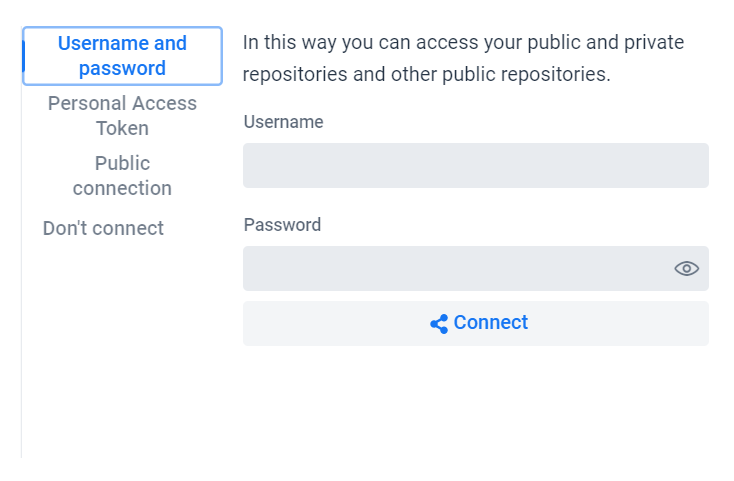
\includegraphics[width=\linewidth]{AnexE-MN-Fig1-1}
%		\caption{Conexión mediante usuario y contraseña}
%		\label{fig:dialogo-conexion_contraseña}
%	\end{subfigure}\hfill
%	\begin{subfigure}{.45\textwidth}
%		\centering
%		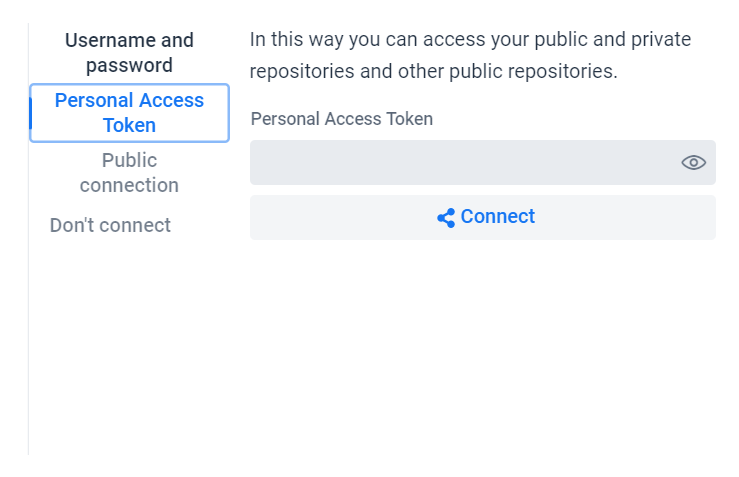
\includegraphics[width=\linewidth]{AnexE-MN-Fig1-2}
%		\caption{Conexión mediante \textit{Personal Access Token}}
%		\label{fig:dialogo-conexion_token}
%	\end{subfigure}
%	\begin{subfigure}{.45\textwidth}
%		\centering
%		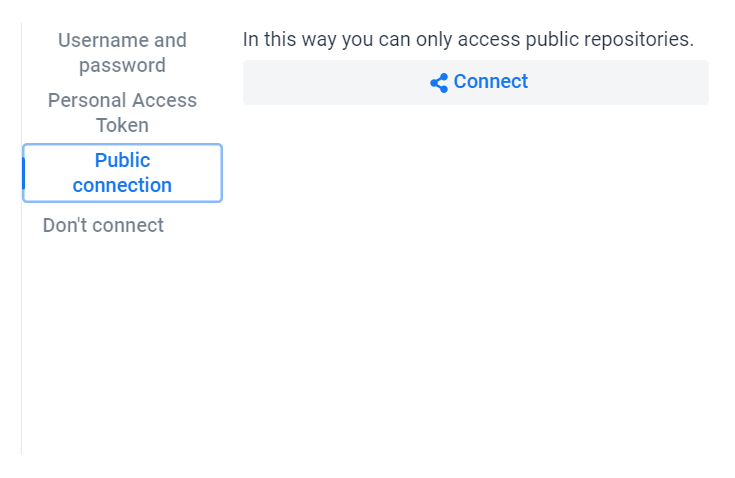
\includegraphics[width=\linewidth]{AnexE-MN-Fig1-3}
%		\caption{Conexión publica}
%		\label{fig:dialogo-conexion_publica}
%	\end{subfigure}\hfill
%	\begin{subfigure}{.45\textwidth}
%		\centering
%		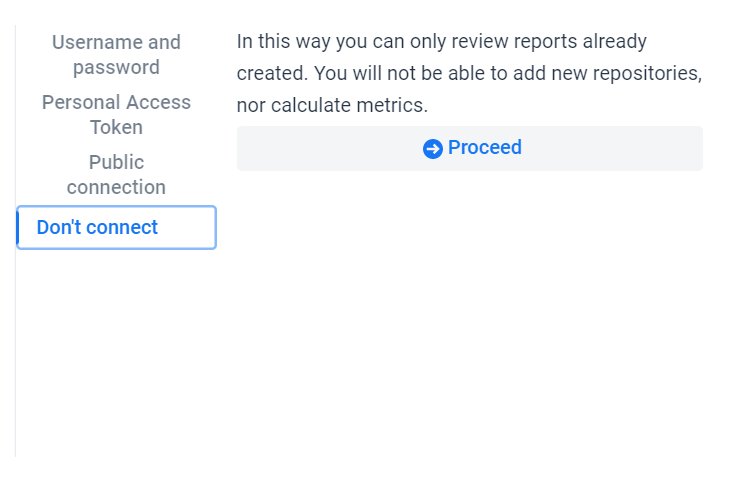
\includegraphics[width=\linewidth]{AnexE-MN-Fig1-4}
%		\caption{Sin conexión}
%		\label{fig:dialogo-conexion_sin-conexion}
%	\end{subfigure}
%	\caption{Distintas formas de establecer una conexión}
%	\label{fig:AnexE-MN-Fig1-}
%\end{figure}
Hay 4 posibilidades, que permiten establecer una conexión con la sesión iniciada (mediante usuario y contraseña o mediante \textit{PA Token}), una conexión pública o utilizar la aplicación sin conexión:
\begin{description}
	\tightlist
	\item[Iniciar sesión en GitLab mediante usuario y contraseña.] Se establece una conexión a GitLab iniciando sesión mediante un nombre de usuario y una contraseña. De esta forma se puede acceder a todos los repositorios públicos y privados accesibles por el usuario. Ver figura \ref{fig:dialogo-conexion_contraseña}.
	\item[Iniciar sesión en GitLab mediante \textit{Personal Access Token}.] Se establece una conexión a GitLab iniciando sesión mediante un \textit{Personal Access Token}. De esta forma se puede acceder a todos los repositorios públicos y privados accesibles por usuario, como ocurría en el caso anterior. 
	Si se accede a GitLab desde una \underline{cuenta externa} a GitLab como Google o GitHub, esta opción es la única manera de iniciar sesión con su cuenta de GitLab. Ver figura \ref{fig:dialogo-conexion_token}.\\
	Para generar un \textit{Personal Access Token} desde GitLab hay que iniciar sesión desde la web y entrar en la configuración del usuario. En el apartado de \textit{Access Token} se debe dar un nombre, opcionalmente una fecha de expiración y los permisos. Para utilizar la aplicación se necesitan estos permisos: \textit{api}, \textit{read\_user}, \textit{read\_repository}, \textit{read\_registry}. Una vez finalizado, pulsar sobre el botón "\textit{Create personal access token}", copiar el token y utilizarlo. Una vez se salga de la ventana en la que se muestra el token, no volverá a aparecer, por lo que se recomienda copiarlo en algún lado. Ver figura \ref{fig:AnexE-MN-Fig2}.
	\imagen{AnexE-MN-Fig2}{Crear un \textit{Personal Access Token} desde GitLab}
	\item[Usar una conexión pública hacia GitLab.] Se establece una conexión pública a GitLab sin iniciar sesión, por lo que solo se podrá acceder a repositorios públicos. Ver figura \ref{fig:dialogo-conexion_publica}.
	\item[No utilizar ninguna conexión.] No se realizará ninguna conexión a GitLab. Solo se podrá trabajar con proyectos y perfil de métricas importados y con el perfil de métricas por defecto. Ver figura \ref{fig:dialogo-conexion_sin-conexion}.
\end{description}

\subsection{Página principal}
\imagen{AnexE-MN-Fig3}{Página principal}
Una vez elegida por primera vez el tipo de conexión deseado se accede a la página principal, como se observa en la figura \ref{fig:AnexE-MN-Fig3}.
\subsubsection{Cambiar el tipo de conexión}
En la parte superior se puede observar el botón de conexión, que indica el tipo de conexión actual.
\begin{itemize}
	\tightlist
	\item Si se ha iniciado sesión mediante usuario y contraseña o mediante un \textit{personal access token}, se mostrará la imágen del usuario y el texto: ``Connected as: <nombre de usuario>''
	\item Si se ha establecido una conexión pública, se mostrara el texto: ``Using a public connection''
	\item Y si no se ha establecido ninguna conexión, el texto mostrado será: ``No connection to GitLab''.
\end{itemize}
Para cambiar el tipo de conexión es obligatorio cerrar, si existe, la conexión actual. Por ello, al pulsar sobre el botón de conexión, se muestra el diálogo de la figura \ref{fig:AnexE-MN-Fig4-1} si existe una conexión y el diálogo de la figura \ref{fig:AnexE-MN-Fig4-2} si no existe conexión. Al pulsar sobre ``\textit{Connect}'' o sobre ``\textit{Close connection}'' se abrirá el diálogo de conexión de las figuras \ref{fig:AnexE-MN-Fig1} y \ref{fig:AnexE-MN-Fig1-}.
%\begin{figure}[!h]
%	\centering
%	\begin{subfigure}{.45\textwidth}
%		\centering
%		
\includegraphics[width=\linewidth]{AnexE-MN-Fig4-1}
%		\caption{Cerrar conexión}
%		\label{fig:AnexE-MN-Fig4-1}
%	\end{subfigure}\hfill
%	\begin{subfigure}{.45\textwidth}
%		\centering
%		
\includegraphics[width=\linewidth]{AnexE-MN-Fig4-2}
%		\caption{Establecer conexión}
%		\label{fig:AnexE-MN-Fig4-2}
%	\end{subfigure}
%	\caption{Modificar tipo de conexión}
%	\label{fig:AnexE-MN-Fig4}
%\end{figure}
\subsubsection{Botón de ayuda}
A la derecha del botón de conexión se encuentra un botón que da acceso a este manual en la Wiki del proyecto.
\subsubsection{Listado de proyectos}
En el centro de la página principal se pueden gestionar los proyectos. Consta de una barra de búsqueda, dos menús, y una tabla que visualiza las métricas de los proyectos que se añadan.

En el cuadro de búsqueda se filtrarán los repositorios por su nombre mientras se vaya escribiendo.

En el menú de ``\textit{Project management}'' existen estas opciones, como se muestra en la figura \ref{fig:AnexE-MN-Fig5-1}:
\begin{itemize}
	\item \textbf{\textit{Add new}.} Permite añadir uno o varios proyectos.
	\item \textbf{\textit{Import}.} Permite importar proyectos a partir de un fichero previamente exportado.
	\item \textbf{\textit{Export}.} Permite exportar todos los proyectos existentes a un fichero, lo que permitirá su posterior importación. Se almacena en un fichero con foromato ``.emr''.
	\item \textbf{\textit{Export to CSV}.} Permite generar un fichero CSV que contenga toda la información de la tabla de proyectos. Este fichero no servirá para importar los proyectos posteriormente.
\end{itemize}
En el menú de ``\textit{Evaluate projects}'' existen estas opciones, como se muestra en la figura \ref{fig:AnexE-MN-Fig5-2}:
\begin{itemize}
	\item \textbf{\textit{Evaluate with new profile}.} Permite evaluar los proyectos calculando los valores mínimos y máximos de cada métrica a partir de los repositorios actuales.
	\item \textbf{\textit{Evaluate with default profile}.} Permite evaluar los proyectos con un perfil por defecto creado a a partir de un conjunto de datos\footnote{\url{https://github.com/clopezno/clopezno.github.io/blob/master/agile_practices_experiment/DataSet_EvolutionSoftwareMetrics_FYP.csv}} de un estudio empírico de las métricas de evolución del software en trabajos finales de grado\cite{lopez_portal_2019}.
	\item \textbf{\textit{Evaluate with imported profile}.} Permite evaluar los proyectos a partir de un perfil de métricas previamente exportado.
	\item \textbf{\textit{Export actual profile}.} Permite exportar el perfil de métricas actual para su posterior importación. Se almacena en un fichero con foromato ``.emmp''.
\end{itemize}
%\begin{figure}[!h]
%	\centering
%	\begin{subfigure}{.45\textwidth}
%		\centering
%		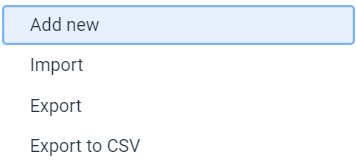
\includegraphics[width=\linewidth]{AnexE-MN-Fig5-1}
%		\caption{Menú: ``\textit{Project management}''}
%		\label{fig:AnexE-MN-Fig5-1}
%	\end{subfigure}\hfill
%	\begin{subfigure}{.45\textwidth}
%		\centering
%		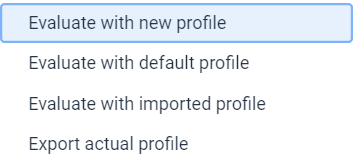
\includegraphics[width=\linewidth]{AnexE-MN-Fig5-2}
%		\caption{Menú: ``\textit{Evaluate projects}''}
%		\label{fig:AnexE-MN-Fig5-2}
%	\end{subfigure}
%	\caption{Menús del listado de repositorios}
%	\label{fig:AnexE-MN-Fig5}
%\end{figure}

La tabla muestra los valores medidos de las métricas para cada proyecto, ver figura \ref{fig:AnexE-MN-Fig8}.
\imagen{AnexE-MN-Fig8}{Tabla que muestra los valores medidos en los proyectos para las métricas}
La tabla presenta las siguientes columnas:
\begin{itemize}
	\item \textbf{Botón de eliminar.} Permite eliminar de la tabla el proyecto seleccionado.
	\item \textbf{\textit{Project}.} Nombre del proyecto con enlace al repositorio de GitLab. Si el nombre es demasiado largo y se corta, se puede utilizar el tooltip que aparece al pasar el ratón por encima del nombre del proyecto.
	\item \textbf{\textit{Date}.} Fecha de la última vez que se obtuvieron las métricas del proyecto.
	\item \textbf{Métricas.} Valor medido de las métricas y un color que evalúa la medida en relación a un perfil de métricas.\\
	Las métricas están clasificadas por categoría: Proceso de orientación (\textit{Process Orientation}) y Constantes de tiempo (\textit{Time Constraints}).\\
	En la cabecera se muestra el nombre de la métrica pero aparecerá la descripción al pasar el puntero del ratón por encima del nombre en forma de tooltip.
	Un \textbf{\underline{perfil de métricas}} es un conjunto de valores mínimo y máximo definidos para cada métrica. Los valores que se encuentran debajo del nombre de las métricas en la cabecera son esos valores mínimo y máximo separados por un guión para su respectiva métrica. En el tooltip se muestra el valor mínimo como Q1 y el valor máximo cómo Q3.
	
	\item \textbf{Botón de recalcular métricas.} Permite volver a obtener las métricas del proyecto (si es posible según la conexión actual a GitLab) y evaluar las nuevas métricas de acuerdo al perfil actual. Se mostrará un mensaje de aviso si se han recalculado correctamente y un mensaje de error en caso contrario.
\end{itemize}


\subsubsection{Añadir un proyecto}
Para añadir un nuevo proyecto, el tipo de conexión deberá ser distinto de ``Sin conexión'' (\textit{No connection to GitLab}), es decir que debe haber una conexión. Seleccionar la opción ``\textit{Add new}'' del menú ``\textit{Project management}'', ver figura \ref{fig:AnexE-MN-Fig5-1}. Se abrirá un diálogo como el de la figura \ref{fig:AnexE-MN-Fig6}. Para \underline{cancelar} se puede pulsar \textit{Esc} o hacer click fuera del diálogo.
%\begin{figure}[!h]
%	\centering
%	\begin{subfigure}{.45\textwidth}
%		\centering
%		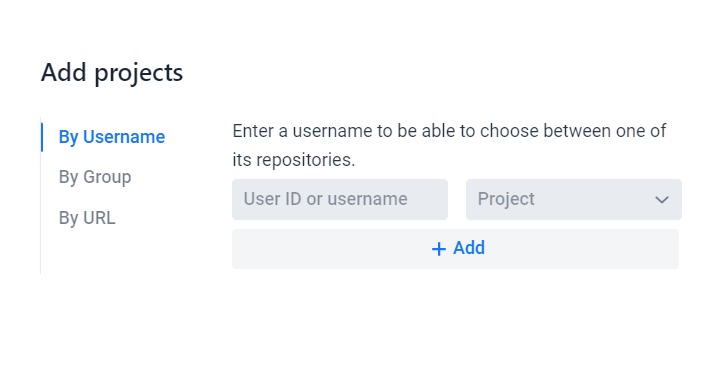
\includegraphics[width=\linewidth]{AnexE-MN-Fig6-1}
%		\caption{Menú: ``\textit{Añadir por pertenencia a usuario}''}
%		\label{fig:AnexE-MN-Fig6-1}
%	\end{subfigure}\hfill
%	\begin{subfigure}{.45\textwidth}
%		\centering
%		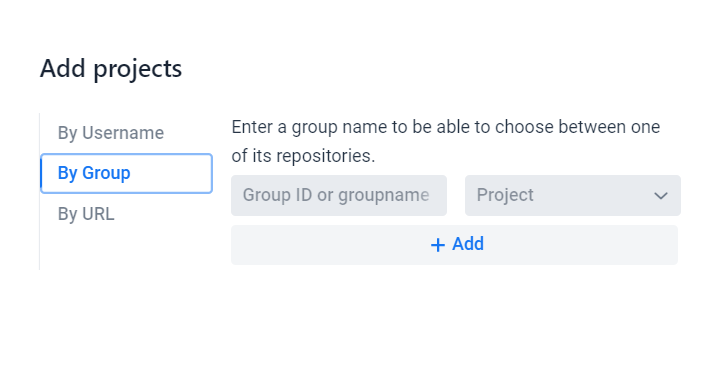
\includegraphics[width=\linewidth]{AnexE-MN-Fig6-2}
%		\caption{Menú: ``\textit{Añadir por pertenencia a grupo}''}
%		\label{fig:AnexE-MN-Fig6-2}
%	\end{subfigure}
%	\begin{subfigure}{.45\textwidth}
%		\centering
%		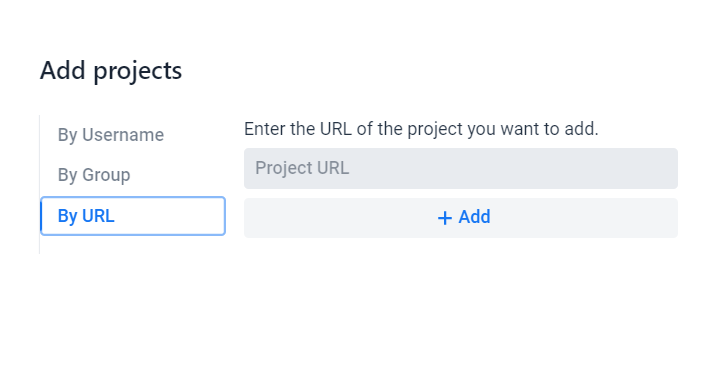
\includegraphics[width=\linewidth]{AnexE-MN-Fig6-3}
%		\caption{Menú: ``\textit{Añadir proyecto por su URL Web}''}
%		\label{fig:AnexE-MN-Fig6-3}
%	\end{subfigure}
%	\caption{Menús del listado de repositorios}
%	\label{fig:AnexE-MN-Fig6}
%\end{figure}
Existen tres posibilidades para añadir un proyecto:
\begin{description}
	\item[Añadir por pertenencia a un usuario.] Se solicita en el campo izquierdo del formulario el nombre de usuario o ID del usuario del cual se desean cargar los proyectos en campo desplegable de la derecha. Se mostrará un mensaje en rojo si el usuario no se existe ``\textit{User not found}'' y un mensaje si el usuario existe ``\textit{User found}'', en ese caso se cargarán todos los proyectos del usuario en el desplegable de la derecha. Seleccionar uno de sus proyectos y pulsar sobre el botón ``\textit{Add}''. Se mostrarán solo los repositorios públicos (incluyendo \textit{forks}) del usuario . No se mostrarán proyectos privados a menos que se haya establecido una conexión con sesión y el usuario especificado en el campo de la izquierda coincida con el usuario que haya iniciado sesión.
	\item[Añadir por pertenencia a un grupo.] El funcionamiento es el mismo que en el caso anterior, con la diferencia de que se solicita el nombre de grupo o ID del grupo en el campo izquierdo. Si el grupo es privado y el tipo de conexión es pública o el usuario que haya iniciado sesión no tiene acceso al grupo, se mostrará un mensaje en rojo de la misma forma que si el grupo no existiera ``\textit{Group not found}''. Si se encuentra el grupo, se mostrará el mensaje ``\textit{Group found}'' y se cargarán todos los proyectos del usuario en el desplegable de la derecha. Seleccionar uno de sus proyectos y pulsar sobre el botón ``\textit{Add}''.
	\item[Añadir por URL Web.] Se solicita la URL Web del proyecto de GitLab. Si no se encuentra (porque no existe o porque con la conexión actual no se tiene acceso al proyecto) se mostrará un mensaje en rojo al pulsar sobre ``\textbf{\textit{Add}}'': ``\textit{Project not found. It doesn't exists or may be inaccessible due to your connection level.}''
\end{description}
Al añadir un nuevo proyecto, se calcularán por primera vez sus métricas y se evaluarán de acuerdo al perfil de métricas actual. Si no se ha creado o importado ningún perfil, se evaluará según el perfil por defecto.
\subsubsection{Importar proyectos}
Los proyectos se pueden importar independientemente del tipo de conexión que exista. Se mostrará un diálogo que permite seleccionar o arrastrar al cuadro un fichero con formato \textit{.emr}, ver figura \ref{fig:AnexE-MN-Fig7}. Se puede seleccionar otro fichero en caso de haber escogido un fichero no deseado. Una vez se cargue el fichero, pulsar sobre ``Import''. Se mostrará un mensaje de error en caso de que el fichero este corrompido (ha sido modificado por una herramienta externa a la aplicación) y no se podrá utilizar ese fichero.
%\begin{figure}[!h]
%	\centering
%	\begin{subfigure}{.45\textwidth}
%		\centering
%		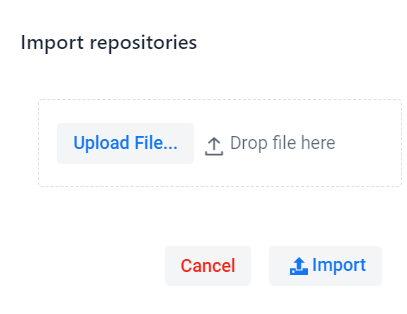
\includegraphics[width=\linewidth]{AnexE-MN-Fig7-1}
%		\caption{Importar repositorios}
%		\label{fig:AnexE-MN-Fig7-1}
%	\end{subfigure}\hfill
%	\begin{subfigure}{.45\textwidth}
%		\centering
%		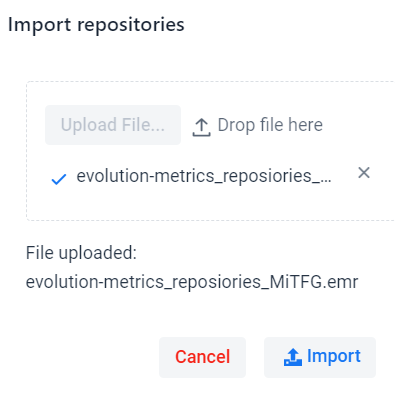
\includegraphics[width=\linewidth]{AnexE-MN-Fig7-2}
%		\caption{Diálogo de importar con fichero cargado}
%		\label{fig:AnexE-MN-Fig7-2}
%	\end{subfigure}
%	\caption{Diálogo para importar repositorios}
%	\label{fig:AnexE-MN-Fig7}
%\end{figure}
\subsubsection{Exportar proyectos}
Para exportar proyectos debe haber al menos un proyecto en la tabla.
Se puede exportar a un fichero \textit{.emr} para su posterior importación o en un fichero \textit{.csv}. Para exportar hay que seleccionar la opción correspondiente en el menú ``\textit{Project management}'', ver figura \ref{fig:AnexE-MN-Fig5-1}. El dialogo para la exportación se muestra en la figura \ref{fig:AnexE-MN-Fig9}. Basta con pulsar sobre ``\textit{Download}'' para poder descargar el fichero.
%\begin{figure}[!h]
%	\centering
%	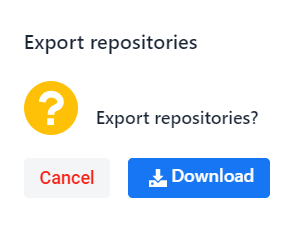
\includegraphics[scale=0.7]{AnexE-MN-Fig9}
%	\caption{Diálogo de exportación}\label{fig:AnexE-MN-Fig9}
%\end{figure}
%\FloatBarrier
\subsubsection{Evaluar los proyectos}
Evaluar un proyecto es evaluar y todas las medidas de las métricas que se realizaron sobre el proyecto en relación a un perfil de métricas en el que se definen los valores mínimos y máximos.\\
El resultado de la evaluación puede ser bueno (la medida se pinta en verde en la tabla), malo (la medida se pinta en rojo) o ``advertencia'' (la medida equivale al valor mínimo o al valor máximo).

Para evaluar un proyecto hay que elegir el perfil de métricas con el que se va a evaluar. Por defecto se coge un perfil de métricas en el que los valores mínimos se corresponden con los quartiles Q1 y los valores máximos con cuartiles Q3 de un conjunto de medidas tomadas sobre TFGs\footnote{\url{https://github.com/clopezno/clopezno.github.io/blob/master/agile_practices_experiment/DataSet_EvolutionSoftwareMetrics_FYP.csv}}\cite{lopez_portal_2019}.

Al evaluar se evalúan todos los proyectos. Se puede elegir el perfil de métricas según la opción elegida en el menú ``\textit{Evaluate projects}'' de la figura \ref{fig:AnexE-MN-Fig5-2}:
\begin{itemize}
	\item \textbf{\textit{Evaluate with new profile}.} Coge como entrada todas las medidas de la tabla y calcula, por cada métrica, los cuartiles Q1 y Q3 para definirlos como valor mínimo y valor máximo de la métrica, respectivamente.
	\item \textbf{\textit{Evaluate with default profile}.} Permite evaluar los proyectos con el perfil por defecto mencionado anteriormente.
	\item \textbf{\textit{Evaluate with imported profile}.} Permite importar el perfil de métricas de un fichero \textit{.emmp}. El perfil se debe haber creado y exportado anteriormente.
\end{itemize}
\subsubsection{Exportar perfil de métricas}
Se puede exportar a un fichero \textit{.emmp} para su posterior importación. Para exportar el perfil de métricas, seleccionar la opción correspondiente del menú ``\textit{Evaluate projects}'' de la figura \ref{fig:AnexE-MN-Fig5-2}: ``\textit{Export actual profile}''. El diálogo para la exportación es similar al de la figura \ref{fig:AnexE-MN-Fig9}. Basta con pulsar sobre ``\textit{Download}'' para poder descargar el fichero que contendrá el perfil de métricas actual.


\bibliographystyle{plain}
\bibliography{bibliografiaAnexos}

\end{document}
